%%%%%%%%%%%%%%%%%%%%%%%%%%%%%%%%%%%%%%%%%%%%%%%%%%%%%%%%%%%%%%%%%%%%%%
%%%%                                                              %%%%
%%%% WISHBONE SD Card Controller IP Core                          %%%%
%%%%                                                              %%%%
%%%% hdl_if.tex                                                   %%%%
%%%%                                                              %%%%
%%%% This file is part of the WISHBONE SD Card                    %%%%
%%%% Controller IP Core project                                   %%%%
%%%% http://opencores.org/project,sd_card_controller              %%%%
%%%%                                                              %%%%
%%%% Description                                                  %%%%
%%%% documentation 'HDL interface' chapter                        %%%%
%%%%                                                              %%%%
%%%% Author(s):                                                   %%%%
%%%%     - Marek Czerski, ma.czerski@gmail.com                    %%%%
%%%%                                                              %%%%
%%%%%%%%%%%%%%%%%%%%%%%%%%%%%%%%%%%%%%%%%%%%%%%%%%%%%%%%%%%%%%%%%%%%%%
%%%%                                                              %%%%
%%%% Copyright (C) 2013 Authors                                   %%%%
%%%%                                                              %%%%
%%%% This source file may be used and distributed without         %%%%
%%%% restriction provided that this copyright statement is not    %%%%
%%%% removed from the file and that any derivative work contains  %%%%
%%%% the original copyright notice and the associated disclaimer. %%%%
%%%%                                                              %%%%
%%%% This source file is free software; you can redistribute it   %%%%
%%%% and/or modify it under the terms of the GNU Lesser General   %%%%
%%%% Public License as published by the Free Software Foundation; %%%%
%%%% either version 2.1 of the License, or (at your option) any   %%%%
%%%% later version.                                               %%%%
%%%%                                                              %%%%
%%%% This source is distributed in the hope that it will be       %%%%
%%%% useful, but WITHOUT ANY WARRANTY; without even the implied   %%%%
%%%% warranty of MERCHANTABILITY or FITNESS FOR A PARTICULAR      %%%%
%%%% PURPOSE. See the GNU Lesser General Public License for more  %%%%
%%%% details.                                                     %%%%
%%%%                                                              %%%%
%%%% You should have received a copy of the GNU Lesser General    %%%%
%%%% Public License along with this source; if not, download it   %%%%
%%%% from http://www.opencores.org/lgpl.shtml                     %%%%
%%%%                                                              %%%%
%%%%%%%%%%%%%%%%%%%%%%%%%%%%%%%%%%%%%%%%%%%%%%%%%%%%%%%%%%%%%%%%%%%%%%
\section{HDL interface}
\label{sec:hdl_if}

    This IP core has a very simple interface:
    \begin{figure}[H]
        \centering
        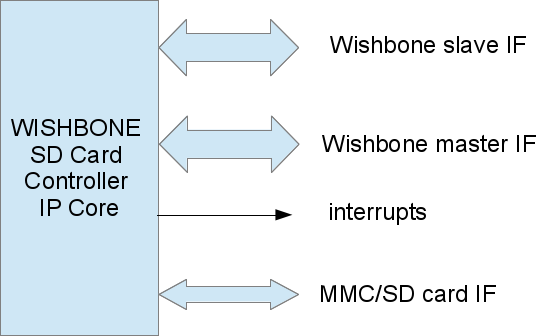
\includegraphics[width=11cm]{../bin/ip_core_if.png}
        % ip_core.png: 384x469 pixel, 96dpi, 10.16x12.41 cm, bb=
        \caption{Wishbone SD Card Controller IP Core interface}
        \label{img:ip_core_if}
    \end{figure}
    The Wishbone slave interface provides access from CPU to all IP core registers (see \ref{sec:regs}). It must
    be connected to a data master. The Wishbone master interface provides access from the DMA engine to RAM (see \ref{sec:dma}). 
    It must be connected to a RAM memory slave. Interrupt signals provide a mechanism to notify the CPU about finished transactions (data and command tranfers).
    They are not necessary for proper operation, if you don't want to use interrupts. The MMC/SD card interface communicates with external MMC/SD cards.
    It must be mapped to external pins of the FPGA which are connected to a MMC/SD card connector. Because those external pins are bidirectional, this IP core
    provides inputs, outputs and output enables for these signals.
    Table \ref{tab:signals} presents all the IP core signals with descriptions.
    
    \begin{table}
    \caption{Description of signals}
        \begin{center}
            \begin{tabular}{l|l|l|l}
                    \rowcolor[gray]{0.7} name & direction & width & description \\ \hline \hline
                    \multicolumn{4}{c}{Wishbone common signals} \\ \hline
                    \texttt{wb\_clk\_i} & input & 1 & clock for both master and slave wishbone transactions \\ \hline
                    \texttt{wb\_rst\_i} & input & 1 & reset for whole IP core \\ \hline
                    \multicolumn{4}{c}{Wishbone slave signals} \\ \hline
                    \texttt{wb\_dat\_i} & input & 32 & data input \\ \hline
                    \texttt{wb\_dat\_o} & output & 32 & data output \\ \hline
                    \texttt{wb\_adr\_i} & input & 32 & address \\ \hline
                    \texttt{wb\_sel\_i} & input & 4 & byte select \\ \hline
                    \texttt{wb\_we\_i} & input & 1 & write enable \\ \hline
                    \texttt{wb\_cyc\_i} & input & 1 & cycle flag \\ \hline
                    \texttt{wb\_stb\_i} & input & 1 & strobe \\ \hline
                    \texttt{wb\_ack\_o} & output & 1 & acknowledge flag \\ \hline
                    \multicolumn{4}{c}{Wishbone master signals} \\ \hline
                    \texttt{m\_wb\_dat\_o} & output & 32 & data output \\ \hline
                    \texttt{m\_wb\_dat\_i} & input & 32 & data input \\ \hline
                    \texttt{m\_wb\_adr\_o} & output & 32 & address \\ \hline
                    \texttt{m\_wb\_sel\_o} & output & 4 & byte select \\ \hline
                    \texttt{m\_wb\_we\_o} & output & 1 & write enable \\ \hline
                    \texttt{m\_wb\_cyc\_o} & output & 1 & cycle flag \\ \hline
                    \texttt{m\_wb\_stb\_o} & output & 1 & strobe \\ \hline
                    \texttt{m\_wb\_ack\_i} & input & 1 & acknowledge flag \\ \hline
                    \texttt{m\_wb\_cti\_o} & output & 3 & cycle type identifier (always 000) \\ \hline
                    \texttt{m\_wb\_bte\_o} & output & 2 & burst type (always 00) \\ \hline
                    \multicolumn{4}{c}{MMC/SD signals} \\ \hline
                    \texttt{sd\_cmd\_dat\_i} & input & 1 & command line input \\ \hline
                    \texttt{sd\_cmd\_out\_o} & output & 1 & command line output \\ \hline
                    \texttt{sd\_cmd\_oe\_o} & output & 1 & command line output enable \\ \hline
                    \texttt{sd\_dat\_dat\_i} & input & 4 & data line inputs \\ \hline
                    \texttt{sd\_dat\_out\_o} & output & 4 & data line outputs \\ \hline
                    \texttt{sd\_dat\_oe\_o} & output & 1 & data line outputs enable \\ \hline
                    \texttt{sd\_clk\_o\_pad} & output & 1 & clock for external MMC/SD card \\ \hline
                    \texttt{sd\_clk\_i\_pad} & input & 1 & clock for MMC/SD interface \\ \hline
                    \multicolumn{4}{c}{Interrupts} \\ \hline
                    \texttt{int\_cmd} & output & 1 & command transaction finished interrupt \\ \hline
                    \texttt{int\_data} & output & 1 & data transaction finished interrupt \\ \hline
                    \hline
            \end{tabular}
            \label{tab:signals}
        \end{center}
    \end{table}     
    
    \subsection{Clock consideration}
    \label{sec:clock}
    
    The IP core needs two clock sources. The first is for Wishbone bus operation (\texttt{wb\_clk\_i}). There are no constraints for this clock. 
    The second is for MMC/SD interface operation (\texttt{sd\_clk\_i\_pad}). 
    \texttt{sd\_clk\_i\_pad} is used to drive the \texttt{sd\_clk\_o\_pad} output, which is the external MMC/SD card clock source, through an internal
    clock divider. This clock divider is able to divide the \texttt{sd\_clk\_i\_pad} clock by 2, 4, 6, 8, ... etc. (2*n where n = [1..256]).
    The \texttt{sd\_clk\_o\_pad} clock frequency depends on the MMC/SD specification. To fully utilize the transmission bandwidth \texttt{sd\_clk\_o\_pad}
    should be able to perform at 25MHz frequency which imposes a minimum constraint of 50MHz on \texttt{sd\_clk\_i\_pad} clock. 
    Clock inputs \texttt{wb\_clk\_i} and \texttt{sd\_clk\_i\_pad} can be sourced by the same signal.
    
    \subsection{DMA engine}
    \label{sec:dma}
    
    The DMA engine is used to lower the CPU usage during data transactions\footnote{"Data transaction" refers to any traffic on the data lines of MMC/SD card interface.}.
    The DMA engine starts its operation immediately after the successful end of any read or write command transactions\footnote{"Command transaction" refers to any traffic on the command line.}
    \footnote{"Read" or "write" commands refer to commands with data payload such as \textit{block read}(CMD17) or \textit{block write}(CMD24).}.
    During write transactions, data is fetched from RAM automatically, starting from a known address. This address has to be configured by the CPU before sending any write commands. 
    Similarly, during read transactions, data is written to RAM automatically, starting from a known address. 
    This address also has to be configured by the CPU before sending any read commands. Because data transmission is half-duplex, 
    read and write addresses are placed in the same configuration register. The function of this register thus depends on the command to be sent.
    
    \subsection{Interrupt generation}
    \label{sec:interrupt}
    
    Interrupts are useful when polling is not an option. There are two interrupt sources: One to signify the end of the command transaction (\texttt{int\_cmd} signal) and
    one to signify the end of the data transaction (\texttt{int\_data} signal). Both interrupts use active high logic. All events that trigger an interrupt can be masked. (see \ref{sec:regs})
    Events which are masked do not participate in interrupt generation(see Fig. \ref{img:events}).
    \begin{figure}[H]
        \centering
        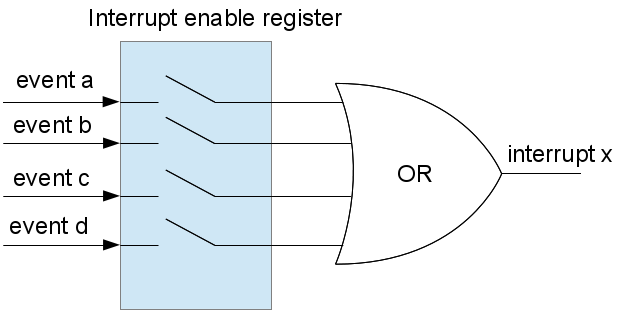
\includegraphics[width=11cm]{../bin/events.png}
        % ip_core.png: 384x469 pixel, 96dpi, 10.16x12.41 cm, bb=
        \caption{Interrupt generation scheme}
        \label{img:events}
    \end{figure}
    
    \subsubsection{Command transaction events}
    \label{sec:cmd_events}

    The command transaction end interrupt is driven in response to command transaction events. The events are:
    \begin{description}
    \item[completion] - transaction completed successfully,
    \item[error] - transaction completed with error (one or more of the following events occurred),
    \item[timeout] - timeout error (the card did not respond in a timely fashion),
    \item[wrong CRC] - CRC check error (CRC calculated from received response data did not match to the CRC field of the response),
    \item[wrong index] - index check error (response consists of wrong index field value).
    \end{description}
    
    \subsubsection{Data transaction events}
    \label{sec:data_events}

    The data transaction end interrupt is driven in response to data transaction events. The events are:
    \begin{description}
    \item[completion] - transaction completed successfully,
    \item[wrong CRC] - CRC check error (in case of write transaction, CRC received in response to write transaction was different than the one calculated by the core; 
    in case of read transaction, the CRC calculated from received data did not match to the CRC field of the received data),
    \item[FIFO error] - internal FIFO error (in case of write transaction, tx FIFO became empty before all data was sent; in case of read transaction, rx FIFO became
    full; both cases are caused by too slow of a wishbone bus or the wishbone bus being busy for too long)).
    \end{description}
    

    